
\documentclass[timesfont]{MITPress-diacriTech-7x9}

\input{xypic}

\begin{document}

\frontmatter

\halftitle{Usable Program Security Analysis}


\begin{seriespage}

\seriestitle{Series Title}

\serieseditor{Series Editor}

\begin{seriesentry}
\item Series entry title
\seriesauthor{Author 1}

\item Series entry title
\seriesauthor{Author 2}

\end{seriesentry}

\end{seriespage}

\booktitle{Usable Program Security Analysis}

\subtitle{Subtitle}


\edition{First Edition}

\edauthor{Marco Pistoia\\
	Omer Tripp
}


\MITimprint{The MIT Press\\
Cambridge, Massachusetts\\
London, England}

\begin{copyrightpage}
$\copyright$ 2009 Massachusetts Institute of Technology\\

All rights reserved. No part of this book may be reproduced in any form or by any electronic or mechanical means
(including photocopying, recording, or information storage and retrieval) without permission in writing from the
publisher.\\

For information about special quantity discounts, please email special sales@mitpress.mit.edu.\\

This book was set in Times Roman and Mathtime Pro 2 by the authors.\\

Printed and bound in the United States of America.\\

Library of Congress Cataloging-in-Publication Data\\

Introduction to algorithms / Thomas H. Cormen $\ldots$ [et al.].�3rd ed.\\
\cindent p. cm.\\

Includes bibliographical references and index.\\
ISBN 978-0-262-03384-8 (hardcover : alk. paper)�ISBN 978-0-262-53305-8 (pbk. : alk. paper)\\
1. Computer programming. 2. Computer algorithms. I. Cormen, Thomas H.\\

QA76.6.I5858 2009\\
005.1�dc22\\

\hspace*{12pc}2009008593\\

10\ 9\ 8\ 7\ 6\ 5\ 4\ 3


\end{copyrightpage}


\dedication{Dedication text}

\begin{epigraphpage}
On 4 April 1980, following a conflict with the Peruvian
government, Fidel Castro ordered the guards posted in front of the Peruvian
embassy in Havana withdrawn. Seizing the chance offered by this absence,
almost 11,000 Cubans stormed into the embassy and demanded political asylum.
Images of a multitude of hungry and thirsty men, women, and children who
were even perched in trees and on the roof of the embassy, were immediately
broadcast worldwide.\source{Source}
\end{epigraphpage}

\tableofcontents

\listoffigures

\listoftables


\begin{contributors}

\name{Thomas H. Cormen}
\affil{Professor and Chair, Department of Computer Science,  Massachusetts Institute of Technology}

\name{Ronald L. Rivest}
\affil{CSAIL, 32 Vassar Street, Room 32-G692, Cambridge MA 02139}


\end{contributors}


\mainmatter



\part{Role of Algorithms}

\chapter{Information-flow Security}


\chapter{The Role of Algorithms in Computing}


\author[1]{Thomas H. Cormen}

\affil[1]{Professor and Chair, Department of Computer Science,  Massachusetts Institute of Technology}

\maketitle

\epigraph{We begin by examining the insertion sort algorithm to solve the sorting problem introduced in
Chapter 1. We define a ``pseudocode'' that should be familiar to you if you have done computer
programming, and we use it to show how we shall specify our algorithms. Having specified the insertion
sort algorithm, we then argue that it correctly sorts, and we analyze its running time. The analysis
introduces a notation that focuses on how that time increases with the number of items to be sorted.
Following our discussion of insertion sort, we introduce the divide-and-conquer approach to the design of
algorithms and use it to develop an algorithm called merge sort. We end with an analysis of merge sort�s
running time.}{Test sentence}


\noindent What are algorithms? Why is the study of algorithms worthwhile? What is the role of algorithms
relative to other technologies used in computers? In this chapter, we will answer these questions.

\Ahead{INTRODUCTION}

This part will start you thinking about designing and analyzing algorithms. It is intended to be a gentle
introduction to how we specify algorithms, some of the design strategies we will use throughout this book,
and many of the fundamental ideas used in algorithm analysis. Later parts of this book will build upon
this base. Chapter 1 provides an overview of algorithms and their place in modem computing systems. This
chapter defines what an algorithm is and lists some examples. It also makes a case that we should consider
algorithms as a technology, alongside technologies such as fast hardware, graphical user interfaces,
object-oriented systems, and networks.

\chapter{Getting Started}

\begin{abstract}
This chapter will familiarize you with the framework we shall use throughout the book to think about the
design and analysis of algorithms. It is self-contained, but it does include several references to
material that we introduce in Chapters 3 and 4. (It also contains several summations, which Appendix A
shows how to solve.)
\end{abstract}



\noindent We begin by examining the insertion sort algorithm to solve the sorting problem introduced in
Chapter 1. We define a ``pseudocode'' that should be familiar to you if you have done computer
programming, and we use it to show how we shall specify our algorithms. Having specified the insertion
sort algorithm, we then argue that it correctly sorts, and we analyze its running time. The analysis
introduces a notation that focuses on how that time increases with the number of items to be sorted.
Following our discussion of insertion sort, we introduce the divide-and-conquer approach to the design of
algorithms and use it to develop an algorithm called merge sort. We end with an analysis of merge sort's
running time.

\section{Insertion Sort}


The numbers that we wish to sort are also known as the \textit{keys}. Although conceptually we are sorting
a sequence, the input comes to us in the form of an array with $n$ elements.

In this book, we shall typically describe algorithms as programs written in a \textit{pseudocode} that is
similar in many respects to $\mathrm{C},\ \mathrm{C}++$, Java, Python, or Pascal. If you have been
introduced to any of these languages, you should have little trouble reading our algorithms. What
separates pseudocode from ``real'' code is that in pseudocode, we employ whatever expressive method is
most clear and concise to specify a given algorithm. Sometimes, the clearest method is English, so do not
be surprised if you come across an English phrase or sentence embedded within a section of ``real'' code.
Another difference between pseudocode and real code is that pseudocode is not typically concerned with
issues of software engineering. Issues data abstraction, modularity, and error handling are often ignored
in order to convey the essence of the algorithm more concisely.


\subsection{The Divide-and-Conquer Approach}

Many useful algorithms are \textit{recursive} in structure: to solve a given problem, they call themselves
recursively one or more times to deal with closely related subproblems. These algorithms typically follow
a \textit{divide-and-conquer} approach: they break the problem into several subproblems that are similar
to the original problem but smaller in size, solve the subproblems recursively, and then combine these
solutions to create a solution to the original problem.


\subsubsection{Order of Growth}

We used some simplifying abstractions to ease our analysis of the INSERTIONSORT procedure. First, we
ignored the actual cost of each statement, using the constants $c_{i}$ to represent these costs. Then, we
observed that even these constants give us more detail than we really need: we expressed the worst-case
running time as $an^{2}+bn+c$ for some constants $a,\ b$, and $c$ that depend on the statement costs
$c_{i}$. We thus ignored not only the actual statement costs, but also the abstract costs $c_{i}$.

We shall now make one more simplifying abstraction: it is the \textit{rate of growth}, or \textit{order of
growth}, of the running time that really interests us. We therefore consider only the leading term of a
formula $(\mathrm{e}.\mathrm{g}.,\ an^{2})$, since the lower-order terms are relatively insignificant for
large values of $n$. We also ignore the leading term's constant coefficient, since constant factors are
less significant than the rate of growth in determining computational efficiency for large inputs. For
insertion sort, when we ignore the lower-order terms and the leading term's constant coefficient, we are
left with the factor of $n^{2}$ from the leading term. We write that insertion sort has a worst-case
running time of $\Theta(n^{2})$ (pronounced ``theta of n-squared``). We shall use $\Theta$-notation
informally in this chapter, and we will define it precisely in Chapter 3.


\paragraph{Analysis of Insertion Sort}

Since the number atoms in the observable universe is estimated to be about $10^{80}$, which is much less
than $2^{65536}$, we rarely encounter an input size $n$ such that $\mathrm{lg}^{*}n>5$. Fibonacci numbers
are related to the \textit{golden ratio} $\phi$ and to its conjugate $\hat{\phi}$, which are the two roots
of the equation.

\subparagraph{Analysis of Merge Sort}


Although the pseudocode for MERGE-SORT works correctly when the number of elements is not even, our
recurrence-based analysis is simplified if we assume that the original problem size is a power of 2. Each
divide step then yields two subsequences of size exactly $n/2$. In Chapter 4, we shall see that this
assumption does not affect the order of growth of the solution to the recurrence.

\subsubparagraph*{Analyzing Divide-and-Conquer Algorithms}

We reason as follows to set up the recurrence for $T(n)$, the worst-case running time of merge sort on $n$
numbers. Merge sort on just one element takes constant time. When we have $n>1$ elements, we break down
the running time as follows.



\section{Asymptotic Notation}

The notations we use to describe the asymptotic running time of an algorithm are defined in terms of
functions whose domains are the set of natural numbers $\mathbb{N}=\{0,1,2,\ \ldots\}$. Such notations are
convenient for describing the worst-case running-time function $T(n)$, which usually is defined only on
integer input sizes. We sometimes find it convenient, however, to \textit{abuse} asymptotic notation in a
variety of ways. For example, we might extend the notation to the domain of real numbers or,
alternatively, restrict it to a subset of the natural numbers. We should make sure, however, to understand
the precise meaning of the notation so that when we abuse, we do not \textit{misuse} it. This section
defines the basic asymptotic notations and also introduces some common abuses.

\begin{theorem}\label{thm1}
For any two functions $f(n)$ and $g(n)$, we have $f(n)=\Theta(g(n))$ if and only if $f(n)=O(g(n))$ and
$f(n)=\Omega(g(n))$. As an example of the application of this theorem, our proof that $an^{2}+bn+c=
\Theta(n^{2})$ for any constants $a, b$, and $c$, where $a>0$, immediately implies that
$an^{2}+bn+c=\Omega(n^{2})$ and $an^{2}+bn+c=O(n^{2})$.
\end{theorem}

In practice, rather than using Theorem~\ref{thm1} to obtain asymptotic upper and lower bounds from
asymptotically tight bounds, as we did for this example, we usually use it to prove asymptotically tight
bounds from asymptotic upper and lower bounds in \ref{cor1}. The looping constructs while, for, and
repeat-until and the if-else conditional construct have interpretations similar to those in $\mathrm{C},\
\mathrm{C}++$, Java, Python, and Pascal. In this book, the loop counter retains its value after exiting
the loop, unlike some situations that arise in $\mathrm{C}++$, Java, and Pascal. We shall use this method
of loop invariants to show correctness later in this chapter and in other chapters as well.

\begin{corollary}\label{cor1}
Prove that the running time of an algorithm is $\Theta(g(n))$ if and only if its worst-case running time
is $O(g(n))$ and its best-case running time is $\Omega(g(n))$.
\end{corollary}

%%
When the first two properties hold, the loop invariant is true prior to every iteration of the loop. (Of
course, we are free to use established facts other than the loop invariant itself to prove that the loop
invariant remains true before each iteration.) We prefer not to get bogged down in such formalism, and so
we rely on our informal analysis to show that the second property holds for the outer loop. We shall use
this method of loop invariants to show correctness later in this chapter and in other chapters as well. We
prefer not to get bogged down in such formalism, and so we rely on our informal analysis to show that the
second property holds for the outer loop. We shall use this method of loop invariants to show correctness
later in this chapter and in other chapters as well in Definition~\ref{defi1}.

\begin{definition}\label{defi1}
For any two functions $f(n)$ and $g(n)$, we have $f(n)=\Theta(g(n))$ if and only if $f(n)=O(g(n))$ and
$f(n)=\Omega(g(n))$. As an example of the application of this theorem, our proof that $an^{2}+bn+c=
\Theta(n^{2})$ for any constants $a, b$, and $c$, where $a>0$, immediately implies that
$an^{2}+bn+c=\Omega(n^{2})$ and $an^{2}+bn+c=O(n^{2})$.
\end{definition}

Note the similarity to mathematical induction, where to prove that a property holds, you prove a base case
and an inductive step. Here, showing that the invariant holds before the first iteration corresponds to
the base case, and showing that the invariant holds from iteration to iteration corresponds to the
inductive step.

\begin{proposition}\label{prop1}
For any two functions $f(n)$ and $g(n)$, we have $f(n)=\Theta(g(n))$ if and only if $f(n)=O(g(n))$ and
$f(n)=\Omega(g(n))$. As an example of the application of this theorem, our proof that $an^{2}+bn+c=
\Theta(n^{2})$ for any constants $a, b$, and $c$, where $a>0$, immediately implies that
$an^{2}+bn+c=\Omega(n^{2})$ and $an^{2}+bn+c=O(n^{2})$.
\end{proposition}

The third property is perhaps the most important one, since we are using the loop invariant to show
correctness.\footnote{Not all authors define the asymptotic notations in the same way, although the
various definitions agree in most common situations. Some of the alternative definitions encompass
functions that are not asymptotically nonnegative, as long as their absolute values are appropriately
bounded. Other properties of elementary mathematical functions can be found in any good mathematical
reference, contain a wealth material on discrete mathematics as used in computer science.} Typically, we
use the loop invariant along with the condition that caused the loop to terminate. The termination
property differs from how we usually use mathematical induction, in which we apply the inductive step
infinitely; here, we stop the ``induction'' when the loop terminates. Let us see how these properties hold
for insertion sort. We start by showing that the loop invariant holds before the first loop iteration.

%%

\begin{lemma}\label{lem1}
For any two functions $f(n)$ and $g(n)$, we have $f(n)=\Theta(g(n))$ if and only if $f(n)=O(g(n))$ and
$f(n)=\Omega(g(n))$. As an example of the application of this theorem, our proof that $an^{2}+bn+c=
\Theta(n^{2})$ for any constants $a, b$, and $c$, where $a>0$, immediately implies that
$an^{2}+bn+c=\Omega(n^{2})$ and $an^{2}+bn+c=O(n^{2})$.
\end{lemma}

We start by showing that the loop invariant holds before the first loop iteration, when $j=2^{1}$ The
subarray $A[1.\ .\ j-1]$, therefore, consists just the single element $A[1]$, which is in fact the
original element in $A[1]$. Moreover, this subarray is sorted (trivially, of course), which shows that the
loop invariant holds prior to the first iteration of the loop.\footnote{It is unlikely that the same constant exactly represents both the time to solve problems of size 1
and the time per array element of the divide and combine steps.}


\begin{assumption}\label{assum1}
For any two functions $f(n)$ and $g(n)$, we have $f(n)=\Theta(g(n))$ if and only if $f(n)=O(g(n))$ and
$f(n)=\Omega(g(n))$. As an example of the application of this theorem, our proof that $an^{2}+bn+c=
\Theta(n^{2})$ for any constants $a, b$, and $c$, where $a>0$, immediately implies that
$an^{2}+bn+c=\Omega(n^{2})$ and $an^{2}+bn+c=O(n^{2})$.
\end{assumption}

A more formal treatment of the second property would require us to state and show a loop invariant for the
while loop of lines 5-7. At this point, however, when the loop is a for loop, the moment at which we check
the loop invariant just prior to the first iteration is immediately after the initial assignment to the
loop-counter variable and just before the first test in the loop header. In the case of INSERTIONSORT,
this time is after assigning 2 to the variable $j$ but before the first test of whether $j\leq A$.
\textit{length}.

\begin{rules}\label{rul1}
For any two functions $f(n)$ and $g(n)$, we have $f(n)=\Theta(g(n))$ if and only if $f(n)=O(g(n))$ and
$f(n)=\Omega(g(n))$. As an example of the application of this theorem, our proof that $an^{2}+bn+c=
\Theta(n^{2})$ for any constants $a, b$, and $c$, where $a>0$, immediately implies that
$an^{2}+bn+c=\Omega(n^{2})$ and $an^{2}+bn+c=O(n^{2})$.
\end{rules}

We prefer not to get bogged down in such formalism, and so we rely on our informal analysis to show that
the second property holds for the outer loop. We shall use this method of loop invariants to show
correctness later in this chapter and in other chapters as well.

\begin{examples}
Prove that the running time of an algorithm is $\Theta(g(n))$ if and only if its worst-case running time
is $O(g(n))$ and its best-case running time is $\Omega(g(n))$.
\end{examples}

Finally, we examine what happens when the loop terminates. The condition causing the for loop to terminate
is that $j>A$. \textit{length} $=n$. Because each loop iteration increases $j$ by 1, we must have $j=n+1$
at that time. Substituting $n+1$ for $j$ in the wording of loop invariant, we have that the subarray
$A[1.\ .n]$ consists of the elements originally in $A[1.\ .n]$, but in sorted order. Observing that the
subarray $A[1.\ .n]$ is the entire array, we conclude that the entire array is sorted. Hence, the
algorithm is correct.

\section{Pseudocode Conventions}

We use the following conventions in our pseudocode.

Indentation indicates block structure. For example, the body of the for loop that begins on line 1
consists of lines 2-8, and the body of the while loop that begins on line 5 contains lines 6-7 but not
line 8. Our indentation style applies to if-else statements as well. Using indentation instead of
conventional indicators of block structure, such as begin and end statements, greatly reduces clutter
while preserving, or even enhancing, clarity.


\begin{remark}
For any two functions $f(n)$ and $g(n)$, we have $f(n)=\Theta(g(n))$ if and only if $f(n)=O(g(n))$ and
$f(n)=\Omega(g(n))$. As an example of the application of this theorem, our proof that $an^{2}+bn+c=
\Theta(n^{2})$ for any constants $a, b$, and $c$, where $a>0$, immediately implies that
$an^{2}+bn+c=\Omega(n^{2})$ and $an^{2}+bn+c=O(n^{2})$.
\end{remark}

The looping constructs while, for, and repeat-until and the if-else conditional construct have
interpretations similar to those in $\mathrm{C},\ \mathrm{C}++$, Java, Python, and Pascal. In this book,
the loop counter retains its value after exiting the loop, unlike some situations that arise in
$\mathrm{C}++$, Java, and Pascal. Thus, \hbox{immediately} after a for loop, the loop counter`s value is
the value that first exceeded the for loop bound. We used this property in our correctness argument for
insertion sort. The for loop header in line 1 is for $j=2$ to \textit{A. length}, and so when this loop
terminates, $j=A. length+1$ (or, equivalently, $j=n+1$, since $n=A$. \textit{length}). We use the keyword
to when a for loop increments its loop counter in each iteration, and we use the keyword downto when a for
loop decrements its loop counter. %When the loop counter changes by an amount greater than 1, the amount of
%change follows the optional keyword by.


\begin{demonstrations}
For any two functions $f(n)$ and $g(n)$, we have $f(n)=\Theta(g(n))$ if and only if $f(n)=O(g(n))$ and
$f(n)=\Omega(g(n))$. As an example of the application of this theorem, our proof that $an^{2}+bn+c=
\Theta(n^{2})$ for any constants $a, b$, and $c$, where $a>0$, immediately implies that
$an^{2}+bn+c=\Omega(n^{2})$ and $an^{2}+bn+c=O(n^{2})$.
\end{demonstrations}


A multiple assignment of the form $i=j=e$ assigns to both variables $i$ and $j$ the value of expression
$e$; it should be treated as equivalent to the assignment $j=e$ followed by the assignment $i=j$.

\begin{solution}
For any two functions $f(n)$ and $g(n)$, we have $f(n)=\Theta(g(n))$ if and only if $f(n)=O(g(n))$ and
$f(n)=\Omega(g(n))$. As an example of the application of this theorem, our proof that $an^{2}+bn+c=
\Theta(n^{2})$ for any constants $a, b$, and $c$, where $a>0$, immediately implies that
$an^{2}+bn+c=\Omega(n^{2})$ and $an^{2}+bn+c=O(n^{2})$.
\end{solution}

Variables (such as $i,\ j$, and \textit{key}) are local to the given procedure. We shall not use global
variables without explicit indication.

\begin{proof}
We use the bounds in Lemma 4.3 to evaluate the summation (4.21) from Lemma 4.2. For case 1, we have
\begin{align*}
T(n) &= \Theta(n^{\log_{b}a})+O(n^{\log_{b}a}) \\
      &= \Theta(n^{\log_{b}a}),
\end{align*}
and for case 2,
\begin{align*}
T(n) &= \Theta(n^{\log_{b}a})+\Theta(n^{\log_{b}a} \mathrm{lg}n)\\
&= \Theta(n^{\log_{b}a}\mathrm{lg}n).
\end{align*}
For case 3,
\begin{align*}
T(n) &= \Theta(n^{\log_{b}a})+\Theta(f(n))\\
     &= \Theta(f(n)),
\end{align*}
because $f(n)=\Omega(n^{\log_{b}a+\epsilon})$.
\end{proof}

We access array elements by specifying the array name followed by the index in square brackets. For
example, $A[i]$ indicates the $i$ th element of the array $A$. The notation ``$\ldots$'' is used to
indicate a range of values within an array. Thus, $A[1\ldots j]$ indicates the subarray of $A$ consisting
of the $j$ elements $A[1],\ A[2],\ \ldots,\ A[j]$.


\section{What Kinds of Problems are Solved by Algorithms?}

\subsection{Numbered Lists}

These lists are far from exhaustive (as you again have probably surmised from this book's heft), but
exhibit two characteristics that are common to many interesting algorithmic problems:
\begin{enumerate}[4.]

\item They have many candidate solutions, the overwhelming majority of which do not solve the problem at hand.
Finding one that does, or one that is ``best,'' can present quite a challenge.

\item
They have practical applications. Of the problems in the above list, finding the shortest path provides
the easiest examples. A transportation firm, such as a trucking or railroad company, has a financial
interest in finding shortest paths through a road or rail network because taking shorter paths results in
lower labor and fuel costs. Or a routing node on the Internet may need to find the shortest path through
the network in order to route a message quickly. Or a person wishing to drive from New York to Boston may
want to find driving directions from an appropriate Web site, or she may use her GPS while driving.

\begin{enumerate}[a.]

\item No black-heights in the tree have changed.

\item No red nodes have been made adjacent. Because $y$ takes $z$'s place in the tree, along with $z$'s color,
we cannot have two adjacent red nodes at $y$'s new position in the tree. In addition, if $y$ was not $z$'s
right child, then $y$'s original right child $x$ replaces $y$ in the tree. If $y$ is red, then $x$ must be
black, and so replacing $y$ by $x$ cannot cause two red nodes to become adjacent.

\item Since $y$ could not have been the root if it was red, the root remains black.

\begin{enumerate}[iii.]

\item
Otherwise, $u=2^{2^{k}}$ for some integer $k\geq 1$, so that $u\geq 4$. In addition to the universe size
$u$, the data structure \textit{pro to-vEB} $(u)$ contains the following attributes, illustrated.

\item An array \textit{cluster} $[0.\ .\ \sqrt{u}-1]$ of $\sqrt{u}$ pointers, each to a \textit{pro to-vEB}
$(\sqrt{u})$ structure.

\item If $u=2$, then it is the base size, and it contains an array $A[0.\ .\ 1]$ of two bits.
\end{enumerate}

\item Since $y$ could not have been the root if it was red, the root remains black.

\end{enumerate}


\item Select a data structure that you have seen previously, and discuss its strengths and limitations.

\item  How are the shortest-path and traveling-salesman problems given above similar? How are they different?
Come up with a real-world problem in which only the best solution will do. Then come up with one in which
a solution that is ``approximately'' the best is good enough.
\end{enumerate}

\subsection{Data Structures}

This book also contains several data structures. A \textit{data structure} is a way to store and organize
data in order to facilitate access and modifications. No single data structure works well for all
purposes, and so it is important to know the strengths and limitations of several of them.

\subsection{Unnumbered Lists}

These lists are far from exhaustive (as you again have probably surmised from this book's heft), but
exhibit two characteristics that are common to many interesting algorithmic problems:
\begin{unlist}
\item They have many candidate solutions, the overwhelming majority of which do not solve the problem at hand.
Finding one that does, or one that is ``best,'' can present quite a challenge.

\item
They have practical applications. Of the problems in the above list, finding the shortest path provides
the easiest examples. A transportation firm, such as a trucking or railroad company, has a financial
interest in finding shortest paths through a road or rail network because taking shorter paths results in
lower labor and fuel costs. Or a routing node on the Internet may need to find the shortest path through
the network in order to route a message quickly.

\end{unlist}

When an algorithm contains a recursive call to itself, we can often describe its running time by a {\it
recurrence equation} or {\it recurrence}, which describes the overall running time on a problem of size
$n$ in terms of the running time on smaller inputs. We can then use mathematical tools to solve the
recurrence and provide bounds on the performance of the algorithm.

\subsection{Bullet List}

Sorting is by no means the only computational problem for which algorithms have been developed. (You
probably suspected as much when you saw the size of this book.) Practical applications of algorithms are
ubiquitous and include the following examples:
\begin{itemize}
\item The Human Genome Project has made great progress toward the goals of identifying all the 100,000 genes in
human DNA, determining the sequences of the 3 billion chemical base pairs that make up human DNA, storing
this information in databases, and developing tools for data analysis.
\begin{itemize}
\item
Each of these steps requires
sophisticated algorithms. Although the solutions to the various problems involved are beyond the scope of
this book, many methods to solve these biological problems use ideas from several of the chapters in this
book, thereby enabling scientists to accomplish tasks while using resources efficiently.

\item The savings are
in time, both human and machine, and in money, as more information can be extracted from laboratory
techniques.
\end{itemize}
\item
The Internet enables people all around the world to quickly access and retrieve large amounts of
information. With the aid of clever algorithms, sites on the Internet are able to manage and manipulate
this large volume of data. Examples of problems that make essential use of algorithms include finding good
routes on which the data will travel.


\item
Electronic commerce enables goods and services to be negotiated and exchanged electronically, and it
depends on the privacy of personal information such as credit card numbers, passwords, and bank
statements. The core technologies used in electronic commerce include public-key \hbox{cryptography} and digital
signatures (covered in Chapter 31), which are based on numerical algorithms and number theory. The savings are
in time, both human and machine, and in money, as more information can be extracted.

\end{itemize}


They have practical applications. Of the problems in the above list, finding the shortest path provides
the easiest examples. A transportation firm, such as a trucking or railroad company, has a financial
interest in finding shortest paths through a road or rail network because taking shorter paths results in
lower labor and fuel costs.

\subsection{Descriptive List}

Our first algorithm, insertion sort, solves the \textit{sorting problem} introduced in Chapter 1:
\begin{descriptive}
\item \head{Input} A sequence of $n$ numbers $\{a_{1},\ a_{2},\ \ldots,\ a_{n})$.


\item \head{Output} A permutation (reordering) $\{a_{1}',\ a_{2}',\ \ldots,\ a_{n}')$ of the input sequence such that
$a_{1}'\leq a_{2}'\geq\cdots\leq a_{n}'$.

\item \head{Divide}
 Divide the n-element sequence to be sorted into two subsequences of $n/2$ elements each.
\end{descriptive}

The numbers that we wish to sort are also known as the \textit{keys}. Although conceptually we are sorting
a sequence, the input comes to us in the form of an array with $n$ elements.

\subsection{List With Heading}

Consider the problem of adding two n-bit binary integers, stored in two n-element arrays $A$ and $B$. The
sum of the two integers should be stored in binary form in an $(n+1)$-element array $C$. State the problem
formally and write pseudocode for adding the two integers.

\listhead{Analyzing Algorithms}

\begin{enumerate}[2.]

\item
Otherwise, $u=2^{2^{k}}$ for some integer $k\geq 1$, so that $u\geq 4$. In addition to the universe size
$u$, the data structure \textit{pro to-vEB} $(u)$ contains the following attributes, illustrated.

\item An array \textit{cluster} $[0.\ .\ \sqrt{u}-1]$ of $\sqrt{u}$ pointers, each to a \textit{pro to-vEB}
$(\sqrt{u})$ structure.

\end{enumerate}


\subsection{Notation}


\begin{notation}[MDA$(H)$]

\item[MDA$(H)$] Maximum domain of attraction of the value distribution $H$

\item[N$(\mu,\sigma^2)$] Gaussian (normal) distribution with mean $\mu$, variance $\sigma^2$

\item[N$(\mu, \Sigma)$] Multivariate Gaussian (normal) distribution with mean vector $\mu$ and covariance
matrix $\Sigma$
\end{notation}




\begin{figure}[b!]
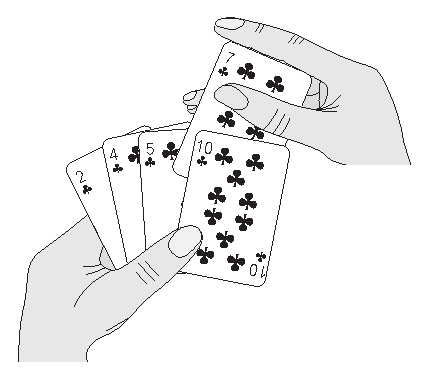
\includegraphics[scale=.85]{fig1}
\caption{Sorting a Hand of Cards Using Insertion Sort.\label{fig1}}%
\end{figure}%

\begin{sidewaysfigure}
 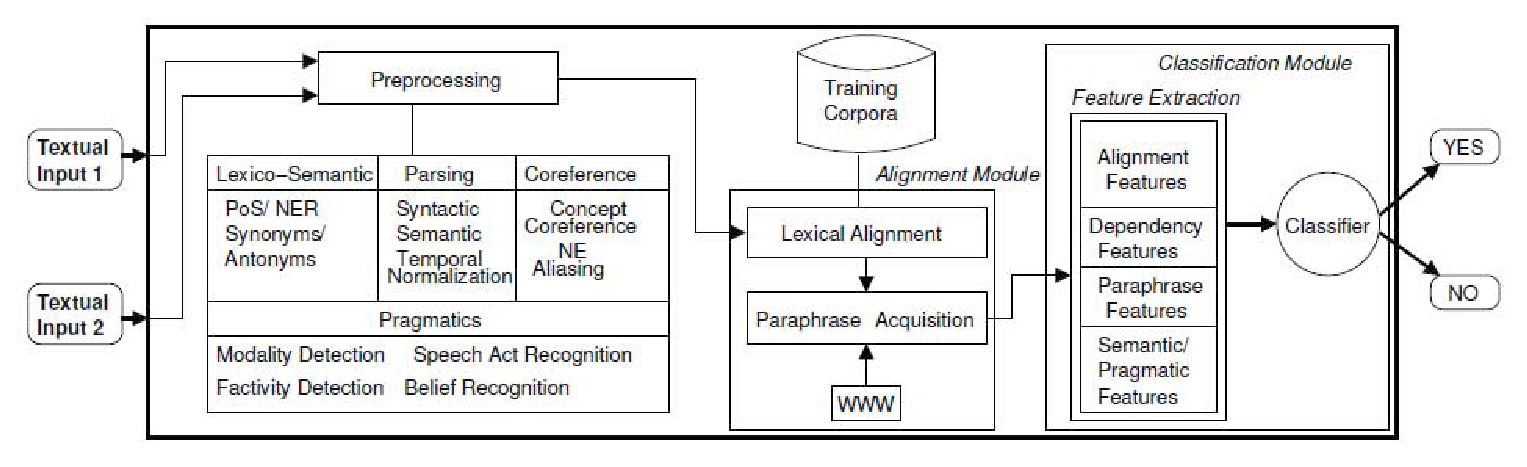
\includegraphics[width=0.9\textwidth]{image-1}\vspace*{-3pt}
\caption{Textual Entailment Framework, as Described. Amount of Time Worked Annually in 7 OECD Countries
Over the Period 1970--2011 (Total Number of Hours Worked During the Year Divided by the Average Number of
Persons of Working Age).} \label{fig:discourse-commits}
\end{sidewaysfigure}

%%%%
\subsection{The Evolution of Participation Rates}\label{ch01:sec1.3}


For each function $f(n)$ and time $t$ in the following table, determine the largest size $n$ of a problem
that can be solved in time $t$, assuming that the algorithm to solve the problem takes $f(n)$
microseconds.


When we evaluated this summation, we attained a bound of $\Theta(n^{2})$ on the worst-case running time of
the algorithm. This example illustrates why you should know how to manipulate and bound summations. In
this equation, the $\Theta$-notation on the left-hand side applies to the variable $k$, but on the
right-hand side, it applies to $n$. We can also apply such manipulations to infinite convergent series.


\section{Arithmetic Series}

\subsection{Extracts}


\begin{extract}
The Human Genome Project has made great progress toward the goals of identifying all the 100,000 genes in
human DNA, determining the sequences of the 3 billion chemical base pairs that make up human DNA, storing
this information in databases, and developing tools for data analysis. Each of these steps requires
sophisticated algorithms. Although the solutions to the various problems involved are beyond the scope of
this book, many methods to solve these biological problems use ideas from several of the chapters in this
book, thereby enabling scientists to accomplish tasks while using resources efficiently. The savings are
in time, and in money, as more information can be extracted from laboratory techniques in
Figures~\ref{fig1} and \ref{fig:discourse-commits}.
\begin{extractlist}

\item They have many candidate solutions, the overwhelming majority of which do not solve the problem at hand.
Finding one that does, or one that is ``best,'' can present quite a challenge.

\item
They have practical applications. Of the problems in the above list, finding the shortest path provides
the easiest examples. A transportation firm, such as a trucking or railroad company, has a financial
interest in finding shortest paths through a road or rail network because taking shorter paths results in
lower labor and fuel costs. Or a routing node on the Internet may need to find the shortest path through
the network in order to route a message quickly. Or a person wishing to drive from New York to Boston may
want to find driving directions from an appropriate Web site, or she may use her GPS while driving.

\item No black-heights in the tree have changed.

\item No red nodes have been made adjacent. Because $y$ takes $z$'s place in the tree, along with $z$'s color,
we cannot have two adjacent red nodes at $y$'s new position in the tree. In addition, if $y$ was not $z$'s
right child, then $y$'s original right child $x$ replaces $y$ in the tree. If $y$ is red, then $x$ must be
black, and so replacing $y$ by $x$ cannot cause two red nodes to become adjacent.

\end{extractlist}

Sorting is by no means the only computational problem for which algorithms have been developed. (You
probably suspected as much when you saw the size of this book.) Practical applications of algorithms are
ubiquitous and include the following examples:
\begin{unlist}
\item An array \textit{cluster} $[0\ldots \sqrt{u}-1]$ of $\sqrt{u}$ pointers, each to a \textit{pro to-vEB}
$(\sqrt{u})$ structure.

\item If $u=2$, then it is the base size, and it contains an array $A[0\ldots 1]$ of two bits.

\item Since $y$ could not have been the root if it was red, the root remains black.

\end{unlist}

With the aid of clever algorithms, sites on the Internet are able to manage and manipulate this large
volume of data. Examples of problems that make essential use of algorithms include finding good routes on
which the data will travel (techniques for solving such problems appear in Chapter 24), and using a search
engine to quickly find pages on which particular information resides (related techniques are in Chapters
11 and 32). This book also contains several data structures. For example, we might need to sort a sequence
of numbers into nondecreasing order. This problem arises frequently in practice and provides fertile
ground for introducing many standard design techniques and analysis tools. Here is how we formally define
the \textit{sorting problem}:
\begin{itemize}
\item
The Internet enables people all around the world to quickly access and retrieve large amounts of
information. With the aid of clever algorithms, sites on the Internet are able to manage and manipulate
this large volume of data. Examples of problems that make essential use of algorithms include finding good
routes on which the data will travel (techniques for solving such problems appear in Chapter 24), and
using a search engine to quickly find pages on which particular information resides (related techniques
are in Chapters 11 and 32). This book also contains several data structures. A {\it data structure} is a
way to store and organize data in order to facilitate access and modifications. No single data structure
works well for all purposes.

\item
Electronic commerce enables goods and services to be negotiated and exchanged electronically, and it
depends on the privacy of personal information such as credit card numbers, passwords, and bank
statements. The core technologies used in electronic commerce include public-key cryptography and digital
signatures (covered in Chapter 31), which are based on numerical algorithms and number theory.
\end{itemize}


The running time of the algorithm is the sum of running times for each statement executed; a statement
that takes $c_{i}$ steps to execute and executes $n$ times will contribute $c_{i}n$ to the total running
time.${}^{\text{6}}$ To compute $T(n)$, the running time of INSERTION-SORT on an input of $n$ values, we
sum the products of the \textit{cost} and \textit{times} columns, obtaining
\[
T(n) = c_{1}n+c_{2}(n-1)+c_{4}(n-1)+c_{5} \sum_{j=2}^{n}t_{j}+c_{6}\sum_{j=2}^{n}(t_{j}-1)
\]

The key operation of the merge sort algorithm is the merging of two sorted sequences in the ``combine''
step. We merge by calling an auxiliary procedure MERGE. $\mathrm{A};p, q, r$), where $A$ is an array and
$p,\ q$, and $r$ are indices into the array such that $p\geq q<r$. The procedure assumes that the
subarrays $A[p.\ .q]$ and $A[q+1.\ .r]$ are in sorted order. It {\it merges} them to form a single sorted
subarray that replaces the current subarray $A[p.\ .r]$.

Even for inputs of a given size, an algorithm`s running time may depend on \textit{which} input of that
size is given. For example, in INSERTION-SORT, the best case occurs if the array is already sorted. For
each $j=2,3, \ldots,\ n$, we then find that $A[i]\leq{}$\textit{key} in line 5 when $i$ has its initial
value of $j-1$. Thus $t_{j}=1$ for $j=2,3, \ldots,\ n$, and the best-case running time is
\begin{numsentence}
\item It is true prior to the first iteration of the loop.

\item If it is true before an iteration of the loop, it remains true before the
next iteration.

\item Apply these principles using data and programs that allowing us to
replicate the main results of the paper of the estimation of labor supply elasticities.

\item
Come up with a real-world problem in which only the best solution will do. Then come up with one in which
a solution that is ``approximately'' the best is good enough.
\end{numsentence}

When the loop is a for loop, the moment at which we check the loop invariant just prior to the first
iteration is immediately after the initial assignment to the loop-counter variable and just before the
first test in the loop header. In the case of INSERTION-SORT, this time is after assigning 2 to the
variable $j$ but before the first test of whether $j\leq A$. \textit{length}. The recursion ``bottoms
out'' when the sequence to be sorted has length 1, in which case there is no work to be done, since every
sequence of length 1 is already in sorted order.

\begin{unnumsentence}
\item No black-heights in the tree have changed  in Table~\ref{time-use}.

\item No red nodes have been made adjacent. Because $y$ takes $z$'s place in the
tree, along with $z$'s color, we cannot have two adjacent red nodes at $y$'s new position in the tree. In
addition, if $y$ was not $z$'s right child, then $y$'s original right child $x$ replaces $y$ in the tree.
If $y$ is red, then $x$ must be black, and so replacing $y$ by $x$ cannot cause two red nodes to become
adjacent.

\end{unnumsentence}

The element $x$, where $0\leq x<u$, is recursively stored in the cluster numbered high $(x)$ as element
low $(x)$ within that cluster.

\end{extract}


\begin{table}[!t]
\processtable{Average Minutes Per Day by Activity and  Employment Status  in the United States in
2003--2006.\label{time-use}}{
\begin{tabular*}{26pc}{@{\extracolsep{\fill}}lcc@{}}
\Toprule & \multicolumn{1}{c}{Employed} & {Unemployed} \\
\Midrule
{Sleep} &  496 &  555 \\
%\Midrule
{Personal care and eating} & 110 & 197 \\
%\Midrule
{Home production, shopping, care of others} & 158 & 254 \\
%\Midrule
{Leisure, travel, sports, and socializing} &  320 & 442\\
%\Midrule
{Work} &  325 & 210 \\
%\Midrule
{Job search} & 321 & 323 \\
\Botrule
\end{tabular*}}{Note: This is where authors provide additional information about
      the data, including whatever notes are needed.
}\vspace*{-3pt}
\end{table}%



Even for inputs of a given size, an algorithm`s running time may depend on \textit{which} input of that
size is given. For example, in INSERTION-SORT, the best case occurs if the array is already sorted. For
each $j=2,3,\ \ldots,\ n$, we then find that $A[i]\leq$ \textit{key} in line 5 when $i$ has its initial
value of $j-1$. Thus $t_{j}=1$ for $j=2,3,\ \ldots,\ n$, and the best-case running time is
\begin{align*}
T(n) &= c_{1}n+c_{2}(n-1)+c_{4}(n-1)+c_{5}(n-1)+c_{8}(n-1)\\
&= (c_{1}+c_{2}+c_{4}+c_{5}+c_{8})n-(c_{2}+c_{4}+c_{5}+c_{8}).
\end{align*}
We can express this running time as $an+b$ for \textit{constants} $a$ and $b$ that depend on the statement
costs $c_{i}$; it is thus a \textit{linear function} of $n$.


If the array is in reverse sorted order--that is, in decreasing order--the worst case results. We must
compare each element $A[j]$ with each element in the entire sorted subarray $A[1\ldots j-1]$, and so
$t_{j}=j$ for $j=2,3, \ldots,\ n$. Noting that
\[
\sum_{j=2}^{n}j=\frac{n(n+1)}{2}-1
\]
and
\[
\sum_{j=2}^{n}(j-1)=\frac{n(n-1)}{2}
\]
(see Appendix A for a review of how to solve these summations), we find that in the worst case, the
running time of INSERTIONSORT is
\begin{align*}
T(n) &= c_{1}n+c_{2}(n-1)+c_{4}(n-1)+c_{5}\left(\frac{n(n+1)}{2}-1\right)\\
&\quad+c_{6}\left(\frac{n(n-1)}{2}\right) +C_{7}\left(\frac{n(n-1)}{2}\right) +c_{8}(n-1)\\
&= \left(\frac{c_{5}}{2}+\frac{c_{6}}{2}+\frac{c_{7}}{2}\right)
n^{2}+\left(c_{1}+c_{2}+c_{4}+\frac{c_{5}}{2}-\frac{c_{6}}{2}-\frac{c_{7}}{2}+c_{8}\right)n\\
&\quad-(c_{2}+c_{4}+c_{5}+c_{8}).
\end{align*}
We can express this worst-case running time as $an^{2}+bn+c$ for constants $a,\ b$, and $c$ that again
depend on the statement costs $c_{i}$; it is thus a \textit{quadratic function} of $n$.

\begin{lstlisting}[language=C]
void initializeMyStruct( myStruct* ms ) {
   static int modulo3 = 0;
   if (modulo3 == 2) {
       modulo3 = 0;
       if (checkDay('tue')) {
           ms->a = 1;
       }
   } else {
       modulo3++;
       ms->a = 0;
   }
}
\end{lstlisting}

An important notational convention we shall adopt is that \textit{logarithm functions will apply only to
the next term in the formula}, so that $\mathrm{lg} n+k$ will mean $\mathrm{lg} n$) $+k$ and not
$\mathrm{lg}(n+k)$. If we hold $b>1$ constant, then for $n>0$, the function $\log_{b}n$ is strictly
increasing.

\subsection{Dialogue}

Given a well-defined notion of the remainder of one integer when divided by another, it is convenient to
provide special notation to indicate equality of remainders. If $(a\ \mathrm{mod}\ n)=(b\mathrm{mod}\ n)$,
we write $a\equiv b(\mathrm{mod}\ n)$ and say that $a$ is \textit{equivalent} to $b$, modulo $n$. In other
words, $a\equiv b(\mathrm{mod}\ n)$ if $a$ and $b$ have the same remainder when divided by $n$.
Equivalently, $a\equiv b(\mathrm{mod}\ n)$ if and only if $n$ is a divisor of $b-a$. We write $a\not\equiv
b(\mathrm{mod}\ n)$ if $a$ is not equivalent to $b$, modulo $n$.
   \begin{dialogue}
     \speak{Vladimir} Whare are all these corpses from?
     \speak{Estragon} These skeletons.
     \speak{Vladimir} A charnel-house!  A charnel-house!
     \speak{Estragon} I'm in hell!
     \speak{Vladimir} Where were you?
     \speak{Estragon} They're coming there too!
     \speak{Vladimir}  We're surrounded! makes a rush  towards back.  Imbecile!  There's no way out there.
                      There!  Not a soul in sight!  Off you go!  Quick!
   \end{dialogue}

For any integer $a$ and any positive integer $n$, the value $a \mathrm{mod}\ n$ is the \textit{remainder}
(or \textit{residue}) of the quotient $a/n$. We can extend our notation to the case of two parameters $n$
and $m$ that can go to infinity independently at different in rates.

\subsection{In Text Table}

For any real number $x$, we denote the greatest integer less than or equal to $x$ by $\lfloor x\rfloor$
(read the floor of $x$) and the least integer greater than or equal to $x$ by $\lceil x\rceil$ (read ``the
ceiling of $x$). For all real $x$,
\begin{table}[!h]
\unprocesstable{}{
\begin{tabular*}{26pc}{@{\extracolsep{\fill}}llccc@{}}
\Toprule
        Stubhead & \( df \) & \( f \) & \( \eta \) & \( p \) \\
\Midrule
                 &     \multicolumn{4}{c}{Spanning text}     \\%[-3pt]
%&\multicolumn{4}{c@{}}{\hrulefill}\\
        Row 1    & 1        & 0.67    & 0.55       & 0.41    \\
        Row 2    & 2        & 0.02    & 0.01       & 0.39    \\
        Row 3    & 3        & 0.15    & 0.33       & 0.34    \\
        Row 4    & 4        & 1.00    & 0.76       & 0.54    \\
\Botrule
     \end{tabular*}}{}
\end{table}


We can extend our notation to the case of two parameters $n$ and $m$ that can go to infinity independently
at different rates. For a given function $g(n,\ m)$, we denote by $O(g(n,\ m))$ the set of functions. For
any integer $a$ and any positive integer $n$, the value $a \mathrm{mod}\ n$ is the \textit{remainder} (or
\textit{residue}) of the quotient $a/n$. We can extend our notation to the case of two parameters $n$ and
$m$ that can go to infinity independently at different in rates.

\boxhead{Common Functions}

\begin{mdframed}
This section reviews some standard mathematical functions and notations and explores the relationships
among them. It also illustrates the use of the asymptotic notations.

As an example of the application of this theorem, our proof $an^{2}+bn+c= \Theta(n^{2})$ for any constants
$a,\ b$, and $c$, where $a>0$, immediately implies that $an^{2}+bn+c=\Omega(n^{2})$ and
$an^{2}+bn+c=O(n^{2})$. In practice, rather than using Theorem 3.1 to obtain asymptotic upper and lower
bounds from asymptotically tight bounds, as we did for this example, we usually use it to prove
asymptotically tight bounds from asymptotic upper and lower bounds. We have already seen how asymptotic notation can be used within mathematical formulas. For example, in
introducing O-notation.

\begin{extract}
Although the solutions to the various problems involved are beyond the scope of this book, many methods to
solve these biological problems use ideas from several of the chapters in this book, thereby enabling
scientists to accomplish tasks while using resources efficiently. The savings are in time, both human and
machine, and in money, as more information can be extracted from laboratory techniques.
\end{extract}

The running time of insertion sort therefore belongs to both $\Omega(n)$ and $O(n^{2})$, since it falls
anywhere between a linear function of $n$ and a quadratic function of $n$. Moreover, these bounds are
asymptotically as tight as possible: for instance, the running time of insertion sort is not
$\Omega(n^{2})$, since there exists an input for which insertion sort runs in $\Theta(n)$ time (e.g., when
the input is already sorted). It is not contradictory, however, to say that the \textit{worst-case}
running time of insertion sort is $\Omega(n^{2})$, since there exists an input that causes the algorithm
to take $\Omega(n^{2})$ time.

We have already seen how asymptotic notation can be used within mathematical formulas. For example, in
introducing O-notation, we wrote $n=O(n^{2})$. We might also write $2n^{2}+3n+1=2n^{2}+\Theta(n)$. How do
we interpret such formulas?
\[
T(n) = c_{1}n+c_{2}(n-1)+c_{4}(n-1)+c_{5} \sum_{j=2}^{n}t_{j}+c_{6}\sum_{j=2}^{n}(t_{j}-1)
\]

When the asymptotic notation stands alone (that is, not within a larger formula) on the right-hand side of
an equation (or inequality), as in $n=O(n^{2})$, we have already defined the equal sign to mean set
membership: $n\in O(n^{2})$. In general, however, when asymptotic notation appears in a formula, we
interpret it as standing for some anonymous function that we do not care to name. For example, the formula
$2n^{2}+3n+1=2n^{2}+\Theta(n)$ means that $2n^{2}+3n+1=2n^{2}+f(n)$, where $f(n)$ is some function in the
set $\Theta(n)$.

Using asymptotic notation in this manner can help eliminate inessential detail and clutter in an equation.
For example, in Chapter 2 we expressed the worst-case running time of merge sort as the recurrence
$T(n)=2T(n/2)+\Theta(n)$.

\section{Insertion Sort}


The numbers that we wish to sort are also known as the \textit{keys}. Although conceptually we are sorting
a sequence, the input comes to us in the form of an array with $n$ elements.

In this book, we shall typically describe algorithms as programs written in a \textit{pseudocode} that is
similar in many respects to $\mathrm{C},\ \mathrm{C}++$, Java, Python, or Pascal. If you have been
introduced to any of these languages, you should have little trouble reading our algorithms. What
separates pseudocode from ``real'' code is that in pseudocode, we employ whatever expressive method is
most clear and concise to specify a given algorithm.


\subsection{The Divide-and-Conquer Approach}

Many useful algorithms are \textit{recursive} in structure: to solve a given problem, they call themselves
recursively one or more times to deal with closely related subproblems. These algorithms typically follow
a \textit{divide-and-conquer} approach: they break the problem into several subproblems that are similar
to the original problem but smaller in size, solve the subproblems recursively, and then combine these
solutions to create a solution to the original problem.


\subsubsection{Order of Growth}

We used some simplifying abstractions to ease our analysis of the INSERTIONSORT procedure. First, we
ignored the actual cost of each statement, using the constants $c_{i}$ to represent these costs. Then, we
observed that even these constants give us more detail than we really need: we expressed the worst-case
running time as $an^{2}+bn+c$ for some constants $a,\ b$, and $c$ that depend on the statement costs
$c_{i}$. We thus ignored not only the actual statement costs, but also the abstract costs $c_{i}$.

We shall now make one more simplifying abstraction: it is the \textit{rate of growth}, or \textit{order of
growth}, of the running time that really interests us. We therefore consider only the leading term of a
formula $(\mathrm{e}.\mathrm{g}.,\ an^{2})$, since the lower-order terms are relatively insignificant for
large values of $n$. We also ignore the leading term's constant coefficient, since constant factors are
less significant than the rate of growth in determining computational efficiency for large inputs. %For
%insertion sort, when we ignore the lower-order terms and the leading term's constant coefficient, we are
%left with the factor of $n^{2}$ from the leading term. We write that insertion sort has a worst-case
%running time of $\Theta(n^{2})$ (pronounced ``theta of n-squared``). We shall use $\Theta$-notation
%informally in this chapter, and we will define it precisely in Chapter 3.


\paragraph{Analysis of Insertion Sort}

Since the number atoms in the observable universe is estimated to be about $10^{80}$, which is much less
than $2^{65536}$, we rarely encounter an input size $n$ such that $\mathrm{lg}^{*}n>5$. Fibonacci numbers
are related to the \textit{golden ratio} $\phi$ and to its conjugate $\hat{\phi}$, which are the two roots
of the equation.


Although the pseudocode for MERGE-SORT works correctly when the number of elements is not even, our
recurrence-based analysis is simplified if we assume that the original problem size is a power of 2. Each
divide step then yields two subsequences of size exactly $n/2$.

\begin{theorem}\label{thm2}
For any two functions $f(n)$ and $g(n)$, we have $f(n)=\Theta(g(n))$ if and only if $f(n)=O(g(n))$ and
$f(n)=\Omega(g(n))$. As an example of the application of this theorem, our proof that $an^{2}+bn+c=
\Theta(n^{2})$ for any constants $a, b$, and $c$, where $a>0$, immediately implies that
$an^{2}+bn+c=\Omega(n^{2})$ and $an^{2}+bn+c=O(n^{2})$.
\end{theorem}


In Chapter 4, we shall see that this assumption does not affect the order of growth of the solution to the
recurrence.

\begin{remark}
For any two functions $f(n)$ and $g(n)$, we have $f(n)=\Theta(g(n))$ if and only if $f(n)=O(g(n))$ and
$f(n)=\Omega(g(n))$. As an example of the application of this theorem, our proof that $an^{2}+bn+c=
\Theta(n^{2})$ for any constants $a, b$, and $c$, where $a>0$, immediately implies that
$an^{2}+bn+c=\Omega(n^{2})$ and $an^{2}+bn+c=O(n^{2})$.
\end{remark}

Since the number atoms in the observable universe is estimated to be about $10^{80}$, which is much less
than $2^{65536}$, we rarely encounter an input size $n$ such that $\mathrm{lg}^{*}n>5$. Fibonacci numbers
are related to the \textit{golden ratio} $\phi$ and to its conjugate $\hat{\phi}$, which are the two roots
of the equation.


\end{mdframed}

The Human Genome Project has made great progress toward the goals of identifying all the 100,000 genes in
human DNA, determining the sequences of the 3 billion chemical base pairs that make up human DNA, storing
this information in databases, and developing tools for data analysis. Each of these steps requires
sophisticated algorithms. Although the solutions to the various problems involved are beyond the scope of
this book, many methods to solve these biological problems use ideas from several of the chapters in this
book, thereby enabling scientists to accomplish tasks while using resources efficiently. The savings are
in time, both human and machine, and in money, as more information can be extracted from laboratory
techniques.


\begin{table}[b!]\vspace*{-6pt}
\processtable{Racial unemployment differences among men aged 16 and older in the United States in
2012.\label{usgapl}} {\begin{tabular*}{\textwidth}{@{\extracolsep{\fill}}lcc@{}}
\Toprule
& \multicolumn{2}{c}{Unemployment Rate} \\
\cline{2-3}
& Annual Average & Ratio with Whites\\
\Midrule
Whites & 7.4 & 1.0 \\
Black or African American & 15\phantom{00} & 2.0 \\
Asian & 5.8 & 0.8 \\
Hispanic or Latino ethnicity & 9.9 & 1.4 \\
\Botrule
\end{tabular*}}{Source: Bureau of Labor Statistics, Labor force statistics from the current population survey, annual averages,
table 24.}
\end{table}%


This section reviews some standard mathematical functions and notations and explores the relationships
among them. It also illustrates the use of the asymptotic notations.

As an example of the application of this theorem, our proof $an^{2}+bn+c= \Theta(n^{2})$ for any constants
$a,\ b$, and $c$, where $a>0$, immediately implies that $an^{2}+bn+c=\Omega(n^{2})$ and
$an^{2}+bn+c=O(n^{2})$. In practice, rather than using Theorem 3.1 to obtain \hbox{asymptotic} upper and
lower bounds from \hbox{asymptotically} tight bounds, as we did for this example, we usually use it to
prove asymptotically tight bounds from asymptotic upper and lower bounds.
When we say that the \textit{running time} (no modifier) of an algorithm is $\Omega(g(n))$, we mean that
\textit{no matter what particular input of size} $n$ \textit{is chosen for each value} $ofn$, the running
time on that input is at least a constant times $g(n)$, for sufficiently large $n$. Equivalently, we are
giving a lower bound on the best-case running time of an algorithm. For example, the best-case running
time of insertion sort is $\Omega(n)$, which implies that the running time of insertion sort is
$\Omega(n)$ in Figure~\ref{usgapl}.

The running time of insertion sort therefore belongs to both $\Omega(n)$ and $O(n^{2})$, since it falls
anywhere between a linear function of $n$ and a quadratic function of $n$. Moreover, these bounds are
asymptotically as tight as possible: for instance, the running time of insertion sort is not
$\Omega(n^{2})$, since there exists an input for which insertion sort runs in $\Theta(n)$ time (e.g., when
the input is already sorted). It is not contradictory, however, to say that the \textit{worst-case}
running time of insertion sort is $\Omega(n^{2})$, since there exists an input that causes the algorithm
to take $\Omega(n^{2})$ time.

We have already seen how asymptotic notation can be used within mathematical formulas. For example, in
introducing O-notation, we wrote $n=O(n^{2})$. We might also write $2n^{2}+3n+1=2n^{2}+\Theta(n)$. How do
we interpret such formulas?

When the asymptotic notation stands alone (that is, not within a larger formula) on the right-hand side of
an equation (or inequality), as in $n=O(n^{2})$, we have already defined the equal sign to mean set
membership: $n\in O(n^{2})$. In general, however, when asymptotic notation appears in a formula, we
interpret it as standing for some anonymous function that we do not care to name. For example, the formula
$2n^{2}+3n+1=2n^{2}+\Theta(n)$ means that $2n^{2}+3n+1=2n^{2}+f(n)$, where $f(n)$ is some function in the
set $\Theta(n)$. In this case, we let $f(n)=3n+1$, which indeed is in $\Theta(n)$.


\backmatter

\begin{exercises}

\begin{enumerate}

\item Express the function $n^{3}/1000-100n^{2}-100n+3$ in terms of O-notation.

\item  Consider sorting $n$ numbers stored in array $A$ by first finding the smallest element of $A$ and
exchanging it with the element in $A[1]$. Then find the second smallest element of $A$, and exchange it
with $A[2]$. Continue in this manner for the first $n-1$ elements of $A$. Write pseudocode for this
algorithm, which is known as \textit{selection sort}. What loop invariant does this algorithm maintain?
Why does it need to run for only the first $n-1$ elements, rather than for all $n$ elements? Give the
best-case and worst-case running times of selection sort in O-notation.
\begin{enumerate}

\item Consider linear search again (see exercise). How many elements of the input sequence need to be
checked on the average, assuming that the element being searched for is equally likely to be any element
in the array? How about in the worst case? What are the average-case and worst-case running times of
linear search in $\Theta$-notation? Justify your answers.

\begin{enumerate}

\item How can we modify almost any algorithm to have a good best-case running time?


\item
Rewrite the MERGE procedure so that it does not use sentinels, instead stopping once either array $L$ or
$R$ has had all its elements copied back to $A$ and then copying the remainder of the other array back
into $A$.


\item
Let $f(n)$ and $g(n)$ be asymptotically nonnegative functions. Using the basic definition of
$\Theta$-notation, prove that $\displaystyle \max(f(n),\ g(n))=\Theta(f(n)+g(n))$.

\end{enumerate}

\item
Show that for any real constants $a$ and $b$, where $b>0$, $(n+a)^{b}=\Theta(n^{b})$.


\item
Show that if $f(n)$ and $g(n)$ are monotonically increasing functions, then so are the functions
$f(n)+g(n)$ and $f(g(n))$, and if $f(n)$ and $g(n)$ are in addition nonnegative, then $f(n)\cdot g(n)$ is
monotonically increasing.

\end{enumerate}
\item
Is the function $\lceil \mathrm{lg}n\rceil$! polynomially bounded? Is the function $\lceil
\mathrm{lglg}n\rceil$ ! polynomially bounded?
\end{enumerate}

Prove by induction that the $i$ th Fibonacci number satisfies the equality $F_{i}=\displaystyle
\frac{\phi^{i}-\hat{\phi}^{i}}{\sqrt{5}}$ where $\phi$ is the golden ratio and $\hat{\phi}$ is its
conjugate.


\section{Insertion Sort}


The numbers that we wish to sort are also known as the \textit{keys}. Although conceptually we are sorting
a sequence, the input comes to us in the form of an array with $n$ elements.

In this book, we shall typically describe algorithms as programs written in a \textit{pseudocode} that is
similar in many respects to $\mathrm{C},\ \mathrm{C}++$, Java, Python, or Pascal. If you have been
introduced to any of these languages, you should have little trouble reading our algorithms. What
separates pseudocode from ``real'' code is that in pseudocode, we employ whatever expressive method is
most clear and concise to specify a given algorithm. Sometimes, the clearest method is English, so do not
be surprised if you come across an English phrase or sentence embedded within a section of ``real'' code.
Another difference between pseudocode and real code is that pseudocode is not typically concerned with
issues of software engineering. Issues data abstraction, modularity, and error handling are often ignored
in order to convey the essence of the algorithm more concisely.


\subsection{The Divide-and-Conquer Approach}

Many useful algorithms are \textit{recursive} in structure: to solve a given problem, they call themselves
recursively one or more times to deal with closely related subproblems. These algorithms typically follow
a \textit{divide-and-conquer} approach: they break the problem into several subproblems that are similar
to the original problem but smaller in size, solve the subproblems recursively, and then combine these
solutions to create a solution to the original problem.


\subsubsection{Order of Growth}

We used some simplifying abstractions to ease our analysis of the INSERTIONSORT procedure. First, we
ignored the actual cost of each statement, using the constants $c_{i}$ to represent these costs. Then, we
observed that even these constants give us more detail than we really need: we expressed the worst-case
running time as $an^{2}+bn+c$ for some constants $a,\ b$, and $c$ that depend on the statement costs
$c_{i}$. We thus ignored not only the actual statement costs, but also the abstract costs $c_{i}$.

We shall now make one more simplifying abstraction: it is the \textit{rate of growth}, or \textit{order of
growth}, of the running time that really interests us. We therefore consider only the leading term of a
formula $(\mathrm{e}.\mathrm{g}.,\ an^{2})$, since the lower-order terms are relatively insignificant for
large values of $n$. We also ignore the leading term's constant coefficient, since constant factors are
less significant than the rate of growth in determining computational efficiency for large inputs. For
insertion sort, when we ignore the lower-order terms and the leading term's constant coefficient, we are
left with the factor of $n^{2}$ from the leading term. We write that insertion sort has a worst-case
running time of $\Theta(n^{2})$ (pronounced ``theta of n-squared``). We shall use $\Theta$-notation
informally in this chapter, and we will define it precisely in Chapter 3.


\paragraph{Analysis of insertion sort}

A better understanding of labor supply behaviors is also key for the design of tax systems in general. The
more sensitive the labor supply to the net wage, the lower the optimal tax rate, because high tax rates
will then tend to shrink the source of taxable income. This sensitivity, also called elasticity, might
vary substantially across gender, age and income groups. Another motivation is the need to analyse
fluctuations of employment over the economic cycle, which depend on how labor supply reacts to changes in
wages. It is assumed that the individual is ready to sacrifice less and less consumption for an extra hour
of leisure when the amount of time dedicated to leisure rises. This property signifies that the marginal
rate of substitution between consumption and leisure diminishes with leisure time, or again that the
indifference curves are convex, which is equivalent to the hypothesis of the quasi-concavity of the
utility function (the relation between the shape of the indifference curves and the utility function is
studied in appendix 1 at the end of this chapter). Note that for a married or cohabiting person, a part of
the income of her partner is capable of being integrated into this set. Thus the budget constraint of the
agent takes the form.


\subparagraph{Analysis of merge sort}


Although the pseudocode for MERGE-SORT works correctly when the number of elements is not even, our
recurrence-based analysis is simplified if we assume that the original problem size is a power of 2. Each
divide step then yields two subsequences of size exactly $n/2$. In Chapter 4, we shall see that this
assumption does not affect the order of growth of the solution to the recurrence.


The notations we use to describe the asymptotic running time of an algorithm are defined in terms of
functions whose domains are the set of natural numbers $\mathbb{N}=\{0,1,2,\ \ldots\}$. Such notations are
convenient for describing the worst-case running-time function $T(n)$, which usually is defined only on
integer input sizes. We sometimes find it convenient, however, to \textit{abuse} asymptotic notation in a
variety of ways. For example, we might extend the notation to the domain of real numbers or,
alternatively, restrict it to a subset of the natural numbers. We should make sure, however, to understand
the precise meaning of the notation so that when we abuse, we do not \textit{misuse} it. This section
defines the basic asymptotic notations and also introduces some common abuses.

\begin{theorem}\label{thm1}
For any two functions $f(n)$ and $g(n)$, we have $f(n)=\Theta(g(n))$ if and only if $f(n)=O(g(n))$ and
$f(n)=\Omega(g(n))$. As an example of the application of this theorem, our proof that $an^{2}+bn+c=
\Theta(n^{2})$ for any constants $a, b$, and $c$, where $a>0$, immediately implies that
$an^{2}+bn+c=\Omega(n^{2})$ and $an^{2}+bn+c=O(n^{2})$.
\end{theorem}

Indentation indicates block structure. For example, the body of the for loop that begins on line 1
consists of lines 2-8, and the body of the while loop that begins on line 5 contains lines 6-7 but not
line 8. Our indentation style applies to if-else statements as well. Using indentation instead of
conventional indicators of block structure, such as begin and end statements, greatly reduces clutter
while preserving, or even enhancing, clarity.


\begin{remark}
For any two functions $f(n)$ and $g(n)$, we have $f(n)=\Theta(g(n))$ if and only if $f(n)=O(g(n))$ and
$f(n)=\Omega(g(n))$. As an example of the application of this theorem, our proof that $an^{2}+bn+c=
\Theta(n^{2})$ for any constants $a, b$, and $c$, where $a>0$, immediately implies that
$an^{2}+bn+c=\Omega(n^{2})$ and $an^{2}+bn+c=O(n^{2})$.
\end{remark}

The looping constructs while, for, and repeat-until and the if-else conditional construct have
interpretations similar to those in $\mathrm{C},\ \mathrm{C}++$, Java, Python, and Pascal. In this book,
the loop counter retains its value after exiting the loop, unlike some situations that arise in
$\mathrm{C}++$, Java, and Pascal. Thus, immediately after a for loop, the loop counter`s value is the
value that first exceeded the for loop bound. We used this property in our correctness argument for
insertion sort. The for loop header in line 1 is for $j=2$ to \textit{A. length}, and so when this loop
terminates, $j=A. length+1$ (or, equivalently, $j=n+1$, since $n=A$. \textit{length}). We use the keyword
to when a for loop increments its loop counter in each iteration, and we use the keyword downto when a for
loop decrements its loop counter. When the loop counter changes by an amount greater than 1, the amount of
change follows the optional keyword by.


\end{exercises}


\setcounter{chapter}{0}
\begin{appendices}
\chapter{Summations}

When an algorithm contains an iterative control construct such as a while or for loop, we can express its
running time as the sum of the times spent on each execution of the body of the loop. For example, we
found in Section 2.2 that the jth iteration of insertion sort took time proportional to $j$ in the worst
case. By adding up the time spent on each iteration, we obtained the summation (or series)
\[
\sum_{j=2}^{n}j.
\]

When we evaluated this summation, we attained a bound of $\Theta(n^{2})$ on the worst-case running time of
the algorithm. This example illustrates why you should know how to manipulate and bound summations.

\section{Summation Formulas and Properties}

Given a sequence $a_{1}, a_{2}, \ldots$ , $a_{n}$ of numbers, where $n$ is a nonnegative integer, we can
write the finite sum $a_{1}+a_{2}+\cdots+a_{n}$ as
\[
\sum_{k=1}^{n}a_k.
\]
If $n=0$, the value of the summation is defined to be $0$. The value of a finite series is always well
defined, and we can add its terms in any order.

Given an infinite sequence $a_{1}, a_{2}, \ldots$ of numbers, we can write the infinite sum
$a_{1}+a_{2}+\cdots$ as
\[
\sum_{k=1}^{\infty}a_k,
\]
which we interpret to mean
\[
\lim_{n\to \infty}\sum_{k=1}^{\infty}a_k.
\]
If the limit does not exist, the series \textit{diverges}; otherwise, it \textit{converges}. The terms of
a convergent series cannot always be added in any order. We can, however, rearrange the terms of an
\textit{absolutely convergent series}, that is, a series $ \sum_{k=1}^{\infty}a_{k}$ for which the series
$\sum_{k=1}^{\infty}|a_{k}|$ also converges.

\subsection{Linearity}

For any real number $c$ and any finite sequences $a_{1}, a_{2}, \ldots$ , $a_{n}$ and $b_{1}, b_{2},
\ldots$ , $b_{n}$,
\[
\sum_{k=1}^{n} (ca_k + b_k) = c \sum_{k=1}^{n} a_k + \sum_{k=1}^{n} b_k.
\]
The linearity property also applies to infinite convergent series.

We can exploit the linearity property to manipulate summations incorporating asymptotic notation. For
example,
\[
\sum_{k=1}^{n} \Theta (f(k)) =\Theta \left( \sum_{k=1}^{n} f(k)\right).
\]
In this equation, the $\Theta$-notation on the left-hand side applies to the variable $k$, but on the
right-hand side, it applies to $n$. We can also apply such manipulations to infinite convergent series.

\subsubsection{Arithmetic Series}

The summation
\[
\sum_{k=1}^{n} k = 1+ 2+\cdots + n.
\]
is an \textit{arithmetic series} and has the value
\begin{align}
\sum_{k=1}^{n} k & = \frac{1}{2} (n+1)\\
=\Theta (n^2).
\end{align}


%%%%%

\paragraph{Sums of squares and cubes}

We have the following summations of squares and cubes:
\begin{align}
\sum_{k=0}^{n} k^2  &= \frac{n(n+1)(2n+1)}{6},\\
\sum_{k=0}^{n} k^3  &=\frac{n^2(n+1)^2}{4}.
\end{align}

\subparagraph*{Geometric series}

For real $x \neq 1$, the summation
\[
\sum_{k=0}^{n} x^k= 1 + x + x^2 +\cdots+ x^n
\]
Because we assume that $0^0 = 1$, these formulas apply even when $x = 0$.

%%%%

Indentation indicates block structure. For example, the body of the for loop that begins on line 1
consists of lines 2-8, and the body of the while loop that begins on line 5 contains lines 6-7 but not
line 8. Our indentation style applies to if-else statements as well. Using indentation instead of
conventional indicators of block structure, such as begin and end statements, greatly reduces clutter
while preserving, or even enhancing, clarity.


\begin{remark}
For any two functions $f(n)$ and $g(n)$, we have $f(n)=\Theta(g(n))$ if and only if $f(n)=O(g(n))$ and
$f(n)=\Omega(g(n))$. As an example of the application of this theorem, our proof that $an^{2}+bn+c=
\Theta(n^{2})$ for any constants $a, b$, and $c$, where $a>0$, immediately implies that
$an^{2}+bn+c=\Omega(n^{2})$ and $an^{2}+bn+c=O(n^{2})$.
\end{remark}

The looping constructs while, for, and repeat-until and the if-else conditional construct have
interpretations similar to those in $\mathrm{C},\ \mathrm{C}++$, Java, Python, and Pascal.${}^{\text{4}}$
In this book, the loop counter retains its value after exiting the loop, unlike some situations that arise
in $\mathrm{C}++$, Java, and Pascal. Thus, immediately after a for loop, the loop counter`s value is the
value that first exceeded the for loop bound.

\begin{theorem}\label{thm1}
For any two functions $f(n)$ and $g(n)$, we have $f(n)=\Theta(g(n))$ if and only if $f(n)=O(g(n))$ and
$f(n)=\Omega(g(n))$. As an example of the application of this theorem, our proof that $an^{2}+bn+c=
\Theta(n^{2})$ for any constants $a, b$, and $c$, where $a>0$, immediately implies that
$an^{2}+bn+c=\Omega(n^{2})$ and $an^{2}+bn+c=O(n^{2})$.
\end{theorem}

In practice, rather than using Theorem~\ref{thm1} to obtain asymptotic upper and lower bounds from
asymptotically tight bounds, as we did for this example, we usually use it to prove asymptotically tight
bounds from asymptotic upper and lower bounds in \ref{cor1}.

\subsection{Extracts}

The Human Genome Project has made great progress toward the goals of identifying all the 100,000 genes in
human DNA, determining the sequences of the 3 billion chemical base pairs that make up human DNA, storing
this information in databases, and developing tools for data analysis. Each of these steps requires
sophisticated algorithms. The Human Genome Project has made great progress toward the goals of identifying all the 100,000 genes in
human DNA, determining the sequences of the 3 billion chemical base pairs that make up human DNA, storing
this information in databases, and developing tools for data analysis. Each of these steps requires
sophisticated algorithms.


\begin{extract}
Although the solutions to the various problems involved are beyond the scope of this book, many methods to
solve these biological problems use ideas from several of the chapters in this book, thereby enabling
scientists to accomplish tasks while using resources efficiently. The savings are in time, both human and
machine, and in money, as more information can be extracted from laboratory techniques.
\end{extract}
Indicate, for each pair of expressions $(A,\ B)$ in the table below, whether $A$ is $O$, $0$, $\Omega$,
$\omega$, or $\Theta$ of $B$. Assume that $k\leq 1$, $\epsilon>0$, and $c>1$ are constants. Your answer
should be in the form of the table with ``yes'' or ``no'' written in each box.

\subsection{The Divide-and-Conquer Approach}

Many useful algorithms are \textit{recursive} in structure: to solve a given problem, they call themselves
recursively one or more times to deal with closely related subproblems. These algorithms typically follow
a \textit{divide-and-conquer} approach: they break the problem into several subproblems that are similar
to the original problem but smaller in size, solve the subproblems recursively, and then combine these
solutions to create a solution to the original problem.


\subsection{Order of Growth}

We used some simplifying abstractions to ease our analysis of the INSERTIONSORT procedure. First, we
ignored the actual cost of each statement, using the constants $c_{i}$ to represent these costs. Then, we
observed that even these constants give us more detail than we really need: we expressed the worst-case
running time as $an^{2}+bn+c$ for some constants $a,\ b$, and $c$ that depend on the statement costs
$c_{i}$. We thus ignored not only the actual statement costs, but also the abstract costs $c_{i}$ to the
original problem.


\subsection{Approach}

Many useful algorithms are \textit{recursive} in structure: to solve a given problem, they call themselves
recursively one or more times to deal with closely related subproblems. These algorithms typically follow
a \textit{divide-and-conquer} approach: they break the problem into several subproblems that are similar
to the original problem but smaller in size, solve the subproblems recursively, and then combine these
solutions to create a solution to the original problem.


\subsection{Growth}

We used some simplifying abstractions to ease our analysis of the INSERTIONSORT procedure. First, we
ignored the actual cost of each statement, using the constants $c_{i}$ to represent these costs. Then, we
observed that even these constants give us more detail than we really need: we expressed the worst-case
running time as $an^{2}+bn+c$ for some constants $a,\ b$, and $c$ that depend on the statement costs
$c_{i}$. We thus ignored not only the actual statement costs, but also the abstract costs $c_{i}$ to the
original problem.

\subsection{Order of Growth}

We used some simplifying abstractions to ease our analysis of the INSERTIONSORT procedure. First, we
ignored the actual cost of each statement, using the constants $c_{i}$ to represent these costs. Then, we
observed that even these constants give us more detail than we really need: we expressed the worst-case
running time as $an^{2}+bn+c$ for some constants $a,\ b$, and $c$ that depend on the statement costs
$c_{i}$. We thus ignored not only the actual statement costs, but also the abstract costs $c_{i}$ to the
original problem.


\subsection{Approach}

Many useful algorithms are \textit{recursive} in structure: to solve a given problem, they call themselves
recursively one or more times to deal with closely related subproblems. These algorithms typically follow
a \textit{divide-and-conquer} approach: they break the problem into several subproblems that are similar
to the original problem but smaller in size, solve the subproblems recursively, and then combine these
solutions to create a solution to the original problem to the original problem.



\end{appendices}

%%
\chapter*{Notes}

\begin{notes}[10.]

\item
Knuth [209] traces the origin of the O-notation to a number-theory text by P. Bachmann in 1892. The
o-notation was invented by E. Landau in 1909 for his discussion of the distribution of prime numbers. The
$\Omega$ and $\Theta$ notations were advocated by Knuth [213] to correct the popular, but technically
sloppy, practice in the literature of using O-notation for both upper and lower bounds. Many people
continue to use the O-notation where the $\Theta$-notation is more technically precise. Further discussion
of the history and development of asymptotic notations appears in works by Knuth [209, 213] and Brassard
and Bratley [54].

\item
Not all authors define the asymptotic notations in the same way, although the various definitions agree in
most common situations. Some of the alternative definitions encompass functions that are not
asymptotically nonnegative, as long as their absolute values are appropriately bounded.


\item Knuth [211] provides an encyclopedic treatment of many sorting algorithms. His
comparison of sorting algorithms (page 381) includes exact step-counting analyses, like the one we
performed here for insertion sort. Knuth�s discussion of insertion sort encompasses several variations of
the algorithm. The most important of these is Shell�s sort, introduced by D. L. Shell, which uses
insertion sort on periodic subsequences of the input to produce a faster sorting algorithm in \cite{1}.


\item Not all authors define the asymptotic notations in the same way, although the
various definitions agree in most common situations. Some of the alternative definitions encompass
functions that are not asymptotically nonnegative \cite{2}, as long as their absolute values are
appropriately bounded.


\item Equation (3.20) is due to Robbins [297]. Other properties of elementary mathematical
functions can be found in any good mathematical reference, such as Abramowitz and Stegun [1] or Zwillinger
[362], or in a calculus book, such as \cite{4} or \cite{3}. Knuth [209] and Graham, Knuth, and Patashnik
[152] contain a wealth of material on discrete mathematics as used in computer science.

\item We use min-heaps to implement min-priority queues in Chapters 16, 23, and 24.
We also give an implementation with improved time bounds for certain operations in Chapter 19 and,
assuming that the keys are drawn from a bounded set of nonnegative integers, Chapter 20.


\item The quicksort procedure was invented by \cite{5}; Hoare�s version appears in
Problem 7-1. The PARTITION procedure given in Section 7.1 is due to N. Lomuto. The analysis in Section 7.4
is due to \cite{10}. Sedgewick [305] and \cite{9} provide a good reference on the details of
implementation and how they matter.

\item The decision-tree model for studying comparison sorts was introduced by Ford
and Johnson [110]. Knuth�s comprehensive treatise on sorting \cite{8} covers many variations on the
sorting problem, including the information-theoretic lower bound on the complexity of sorting given here.
Ben-Or [39] studied lower bounds for sorting using generalizations of the decision-tree model.

\item The origin of stacks and queues as data structures in computer science is unclear,
since corresponding notions already existed in mathematics and paper-based business practices before the
introduction of digital computers. Knuth [209] cites A. M. Turing for the development of stacks for
subroutine linkage in 1947.

\item Carter and Wegman introduced the notion of universal classes of hash functions
in 1979 [58].
\end{notes}

\chapter*{Glossary}

\begin{glossary}

\item[formula] A mathematical expression

\item[latex] Is a mark up language specially suited for scientific documents. Turing for the development of stacks for
subroutine linkage

\item[mathematics] Mathematics is what mathematicians do Is a mark up language specially suited for scientific documents. Turing for the development of stacks for
subroutine linkage

\end{glossary}



\begin{thebibliography}{11}

\bibitem{1} Milton Abramowitz and Irene A. Stegun, editors. Handbook of Mathematical Functions.
Dover, 1965.

\bibitem{2} G. M. Adel�fson-Vel�fski.. and E. M. Landis. An algorithm for the organization of information.
Soviet Mathematics Doklady, 3(5):1259.1263, 1962.

\bibitem{3} Alok Aggarwal and Jeffrey Scott Vitter. The input/output complexity of sorting and related
problems. Communications of the ACM, 31(9):1116.1127, 1988.

\bibitem{4} Manindra Agrawal, Neeraj Kayal, and Nitin Saxena. PRIMES is in P. Annals of Mathematics,
160(2):781.793, 2004.

\bibitem{5} Alfred V. Aho, John E. Hopcroft, and Jeffrey D. Ullman. The Design and Analysis of
Computer Algorithms. Addison-Wesley, 1974.

\bibitem{6} Alfred V. Aho, John E. Hopcroft, and Jeffrey D. Ullman. Data Structures and Algorithms.
Addison-Wesley, 1983.

\bibitem{7} Ravindra K. Ahuja, Thomas L. Magnanti, and James B. Orlin. Network Flows: Theory,
Algorithms, and Applications. Prentice Hall, 1993.

\bibitem{8} Ravindra K. Ahuja, Kurt Mehlhorn, James B. Orlin, and Robert E. Tarjan. Faster algorithms
for the shortest path problem. Journal of the ACM, 37(2):213.223, 1990.

\bibitem{9} Ravindra K. Ahuja and James B. Orlin. A fast and simple algorithm for the maximum flow
problem. Operations Research, 37(5):748.759, 1989.

\bibitem{10} Ravindra K. Ahuja, James B. Orlin, and Robert E. Tarjan. Improved time bounds for the
maximum flow problem. SIAM Journal on Computing, 18(5):939.954, 1989.

\bibitem{11} Mikl�Los Ajtai, Nimrod Megiddo, and Orli Waarts. Improved algorithms and analysis for
secretary problems and generalizations. In Proceedings of the 36th Annual Symposium on
Foundations of Computer Science, pages 473.482, 1995.

\end{thebibliography}


\begin{theindex}

\item AA-tree, 338
\item abelian group, 940
\item ABOVE, 1024
\item absent child, 1178
\item absolutely convergent series, 1146
\item absorption laws for sets, 1160
\item abstract problem, 1054
\item acceptable pair of integers, 972
\item acceptance
\subitem by an algorithm, 1058
\subitem by a finite automaton, 996
\item accepting state, 995
\item accounting method, 456�459
\subitem for binary counters, 458
\subitem for dynamic tables, 465�466
\subitem for stack operations, 457�458, 458 ex.
\subitem minimum spanning, see minimum spanning tree
\subitem optimal binary search, 397�404, 413
\item Ackermann�s function, 585
\item activity-selection problem, 415�422, 450

\indexspace

\item babyface, 602 ex.
\item back edge, 609, 613
\item back substitution, 817
\item BAD-SET-COVER-INSTANCE, 1122 ex.
\item BALANCE, 333 pr.
\item balanced search tree
\subitem AA-trees, 338
\subitem AVL trees, 333 pr., 337
\subitem B-trees, 484�504
\item base case, 65, 84
\item base, in DNA, 391
\item basic feasible solution, 866

\indexspace

\item cache hit, 449 pr.
\item cache miss, 449 pr.
\item cache obliviousness, 504
\item caching, off-line, 449 pr.
\item call
\subitem in a multithreaded computation, 776
\subitem of a subroutine, 23, 25 n.
\subitem by value, 21
\item call edge, 778
\item cancellation lemma, 907

\indexspace

\item unary, 1056
\item unbounded linear program, 851
\item unconditional branch instruction, 23
\item uncountable set, 1161
\item underdetermined system of linear equations, 814
\item underflow
\subitem of a queue, 234
\subitem of a stack, 233
\item undirected graph, 1168

\end{theindex}




\end{document}
